\chapter*{Appendices}
\setcounter{section}{0}

\addcontentsline{toc}{chapter}{Appendices}
\renewcommand{\thesection}{\Alph{section}}
In this chapter we review all of the necessary mathematics. A knowledge of multivariable calculus and basic probability theory however, is assumed.\section{Mathematical Preliminaries}
\label{appendix_a}
\subsection{Sets}
Let's start with a central concept of belonging. If $x$ belongs to $A$, then we say that $x$ is an element of $A$ i.e. $x$ is contained in $A$, we can the write it as 
\begin{equation}
    x \in A
\end{equation}
\subsubsection{The Axiom of Extension}
\begin{tcolorbox}
    Two sets are equal if and only if they have the same elements
\end{tcolorbox}
Essentially a set, is determined by its extension. Let's say $A$ and $B$ sets, and that every element of $B$ is also an element of $A$, we then call $B$ a subset of $A$, or $A$ inlucdes $B$
\begin{equation}
    B \subset A
\end{equation}
This does not omit the fact that $A \subset A$ holds true despite being trivial, we term this relation to be reflexive i.e. of relating an element to itself. We can then also term equality to be reflexive. However if A and B are sets such that $B \subset A$ and $B \neq A$, the we term $B$ to be a proper subset of $A$. An interesting thing to .think of then is that if $B \subset A$ and $C \subset B$, the we can say that $C \subset A$. This property of a relation is reflexive. Also, inclusion is antisymmetric i.e. $B \subset A \nrightarrow A \subset B$ whereas equality is symmetric i.e. if $A = B$, then necessarily $B =A$.We can then write down the axiom of extension slightly differently
\begin{tcolorbox}
If $A$ and $B$ are sets, then a necessary and sufficient condition for $A = B$ is that both $B \subset A$ and $A \subset B$ hold true
\end{tcolorbox}
It is also interesting to note that belonging and inclusion are conceptually different despite sounding similar: inclusion is always reflexive whereas it is not always clear if belonging is so.
\subsubsection{The Axiom of Specification}
There are two types of "atomic" statements from which the rest can be constructed:
\begin{itemize}
    \item Assertions of belonging: $x \in A$
    \item Assertions of equality: $A = B$
\end{itemize}
We can construct more complicated sentences out of these using logical operators
\begin{center}
\begin{tabularx}{0.99\textwidth} { 
		| >{\raggedright\arraybackslash}X 
		| >{\centering\arraybackslash}X 
		| >{\raggedleft\arraybackslash}X | }
	\hline
\textbf{Operator} & \textbf{Symbol}\\
	\hline
	And & $\wedge$\\
	\hline
	Or (in the sense of either/both)   & $\vee$\\
	\hline
	Not   & $\lnot$ \\
	\hline
	If-then- (or implies) & $\Rightarrow$\\
	\hline
	If and only if (or equivalent to) & $\Leftrightarrow$\\
	\hline
	For some (or there exists) & $\exists$ \\
	\hline
	For all & $\forall$ \\
	\hline
\end{tabularx}
			\end{center}
There are however a few rules to combine them:
\begin{enumerate}[I]
    \item 
    The not comes before a statement which is enclosed in parantheses \footnote{This is done to avoid ambiguity}
    \item And, or and "if and only if" operators are sandwiched between two sentences and the result is enclosed in brackets
    \item 
    \item 
\end{enumerate}
We can now state a major principle of set theory
\begin{tcolorbox}
    \textit{\textbf{Aussonderungsaxiom:}}\textbf{The Axiom of Specification} \\
    For every set $A$ and to every condition/statement $S(x)$ there corresponds a set $B$ whose elements are exactly those elements $x$ of $A$ for which $S(x)$ hold
    \begin{equation}
        B = \left{x \in A: S(x) \right}
    \end{equation}
\end{tcolorbox}
We can illustrate

The moral? To specify a set, it simply not enough to 
\subsubsection{Unordered Pairs}
\subsubsection{Unions and Intersections}
\subsubsection{Complements and Powers}
\subsubsection{Ordered Pairs}
  \subsubsection{Relations}
\subsubsection{Maps}
\subsubsection{Families}
\subsubsection{Inverses and Composites}
\subsubsection{Order}
\subsubsection{Cartesian Product}
Here the symbol "$\times$" means \textbf{"Cartesian Product"} i.e. it's action w.r.t two sets $\mathbb{A}$ and $\mathbb{B}$ is the set of all ordered pairs $(a, b)$ where $a \in \mathbb{A}$ and $b \in \mathbb{B}$

\subsection{Complex Numbers}
\label{appendix_a}
A complex number is an ordered pair $z = \{a,b\} \in \mathbb{C}$ where $a,b \in \mathbb{R}$ where we can denote it as $z = a + ib$ where $i = \sqrt{-1}$
\subsubsection{Addition}
$z_{1} = a_{1} + ib_{1}, \ z_{2} = a_{2} + ib_{2}$
$$z_{1} + z_{2} =  (a_{1} + a_{2}) + i(b_{1} + b_{2})$$
\subsubsection{Multiplication}
$z_{1} = a_{1} + ib_{1}, \ z_{2} = a_{2} + ib_{2}$
$$z_{1}z_{2} =  (a_{1} + ib_{1})(a_{2} + ib_{2}) = (a_{1}a_{2} - b_{1}b_{2}) + i(a_{1}b_{2} + a_{2}b_{1})$$
\subsubsection{Properties}\footnote{$\mathcal{W}, \mathcal{Z}, \lambda \in \mathbb{C}$}
\subsubsubsubsection{Commutativity}
$$\mathcal{W} + \mathcal{Z} = \mathcal{Z} + \mathcal{W}$$
$$\mathcal{W}\mathcal{Z} = \mathcal{Z}\mathcal{W}$$
\subsubsubsubsection{Associativity}
$$(\mathcal{Z}_1 + \mathcal{Z}_2) + \mathcal{Z}_3 = \mathcal{Z}_1 + (\mathcal{Z}_2 + \mathcal{Z}_3)$$
$$(\mathcal{Z}_1\mathcal{Z}_2)\mathcal{Z}_3 = \mathcal{Z}_1(\mathcal{Z}_2\mathcal{Z}_3)$$
\subsubsection{Identities}
$$\mathcal{Z} + 0 = \mathcal{Z}$$
$$\mathcal{Z}1 = \mathcal{Z}$$
\subsubsubsubsection{Additive Inverse}
$$\forall \ \mathcal{Z} \ \exists \ \mathcal{Z}^{-1} \ | \ \mathcal{Z} + \mathcal{Z}^{-1} = 0$$
\subsubsubsubsection{Multiplicative Inverse}
$$\forall \  \mathcal{Z} \neq 0 \ \exists \ \mathcal{W} \ | \ \mathcal{Z}\mathcal{W} = 1$$
\subsubsubsubsection{Distributive Property}
$$\lambda(\mathcal{W} + \mathcal{Z}) = \lambda\mathcal{W} + \lambda\mathcal{Z}$$



\section{Fourier Analysis}
Fourier analysis is the study of a special set of an integral transforms. 
A fourier series is the decomposition of a general wave or oscillation into harmonic components.
Because we treat the wave vector as the independent variable of a wave, the Fourier decomposition
is typically done in terms of wave vectors. A Fourier series is a sum of sinusoidal functions, each of
which is a harmonic of some fundamental wave vector or spatial frequency. A Fourier transform is an
integral over a continuous distribution of sinusoidal functions.
A Fourier series is appropriate when the system has boundary conditions that limit the allowed
wave vectors to a discrete set. For a system where the spatial periodicity is $2L$, the Fourier decomposition of a general periodic function is the series
\begin{equation}
f(x) = \sum_{-\infty}^{\infty} c_{n}e^{i k_{n}x}
\end{equation}
where,
$$k_{n} = \frac{n \pi}{L}$$
Here $c_{n} \in \mathbb{C}$. All $f(x) \in \mathbb{R}$ can be written as:
\begin{equation}
f(x) = \frac{a_{0}}{2} + \sum^{\infty}_{n=1} \left[a_{n}\cos \left(\frac{n \pi x}{L} \right) + b_{n}\sin \left(\frac{n \pi x}{L}\right) \right]
\end{equation}
Where,
\begin{equation}
	a_{n} = \frac{1}{L} \int_{0}^{2L} f(x) \cos\left(\frac{n \pi x}{L}\right) dx
\end{equation}
\begin{equation}
	b_{n} = \frac{1}{L} \int_{0}^{2L} f(x) \sin\left(\frac{n \pi x}{L}\right) dx
\end{equation}
\begin{equation}
	c_{n} = \frac{1}{2L} \int_{0}^{2L} f(x) e^{-ik_{n}x}dx
\end{equation}
obtained by calculating the overlap integrals (i.e., projections or inner products) of the desired function with the harmonic basis functions. That is provided $f(x)$, obeys the following conditions i.e. \textbf{Dirichlet conditions}:
\begin{itemize}
\item It must be absolutely integrable over a period.
\item It must be of bounded variation in any given bounded interval.
\item It must have a finite number of discontinuities in any given bounded interval, and the discontinuities cannot be infinite.
\end{itemize}
A Fourier transform is appropriate when the system has no boundary conditions that limit the allowed wave vectors. In this case, the Fourier decomposition is an integral over a continuum of wave vectors:
\begin{equation}
	f(x) = \frac{1}{\sqrt{2 \pi}} \int_{-\infty}^{\infty} a(k)e^{ikx}dk
\end{equation}
where  the  expansion  function  $a(k)$  is  complex. To  obtain  the  expansion  function  $a(k)$  for  a  givenspatial function $f(x)$ requires the inverse Fourier transform
\begin{equation}
	a(k) = \frac{1}{\sqrt{2 \pi}} \int_{-\infty}^{\infty} f(x)e^{-ikx}dx
\end{equation}
which is a projection of the spatial function $f(x)$ onto the harmonic basis functions $e^{ikx}/\sqrt{2 \pi}$. The basis functions are orthogonal and normalized in the Dirac sense, which means their projections onto each other are Dirac delta functions
\begin{equation}
\begin{split}
	\frac{1}{2 \pi} & \int_{-\infty}^{\infty} e^{ik^{'}x}e^{-ikx}dx = \delta(k-k^{'})\\
	\frac{1}{2 \pi} & \int_{-\infty}^{\infty} e^{ikx^{'}}e^{-ikx}dk = \delta(x-x^{'})
\end{split}
\end{equation}
\subsection{Parseval’s theorem}
Parseval’s theorem states that the power is the same whether calculated in position space or wave-vector space:
\begin{equation}
\int^{\infty}_{-\infty} \abs{f(x)}^{2}dx = \int^{\infty}_{-\infty} \abs{a(k)}^{2}dk
\end{equation}

\section{The Dirac Delta Function}
\subsection{The Divergence of $\frac{\hat{r}}{r^{2}}$}
We can see why the divergence is,
\begin{equation}
\nabla . \frac{\hat{r}}{r^{2}} = 0
\end{equation}
But if we calculate this using the Divergence theorem, we find that ,
\begin{equation}
	\oint v .da = \int \left( \frac{\hat{r}}{r^{2}} \right) . \left( r^{2} \sin(\theta) d \theta d \phi \hat{r} \right) = \left( \int_{0}^{\pi} \sin(\theta) d \theta \right) \left( \int_{0}^{2\pi} d \phi \right) = 4 \pi
\end{equation}
This is paradoxical. The issue is that it blows up at $r=0$ but is is neglible everywhere else. How do we fix this? The Dirac Delta functional!
\subsection{The One-Dimensional Dirac Delta Functional}
The Dirac Delta is a functional \footnote{An object that is a map between functions} which we define as,
\begin{equation} \label{deltadef}
\delta(x-a)= 
\begin{cases}
0, & \text{if } x \neq a\\
\infty,              & \text{if } x = a
\end{cases}
\end{equation}
\begin{equation}
\int_{- \infty}^{+ \infty} \delta(x-a) dx = 1
\label{del2}
\end{equation}
$\forall \  a \in \mathbb{R}$
We can visualize it as a sharp peak at $a$,
\begin{figure}[!ht]
	\centering
	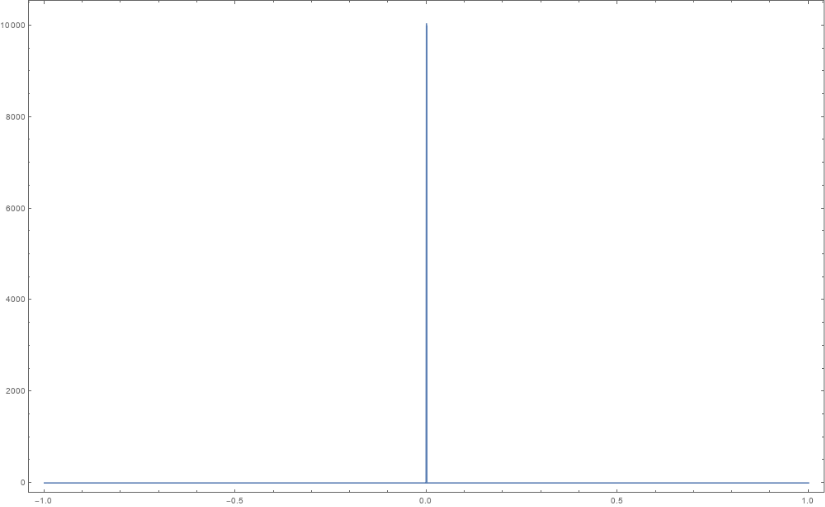
\includegraphics[scale=0.5]{Figures/delta-distribution.png}
	\caption{A Plot of $\delta(x)$}
\end{figure}
We can interpret \ref{del2} as saying "the area of the delta distribution is always 1".
\begin{equation}
f(x)\delta(x - a ) = f(a)
\end{equation}
We can combine these to get,
\begin{equation}
\int_{- \infty}^{+ \infty} \delta(x-a) f(x) dx = f(a)
\end{equation}
\subsubsection{A few interesting properties}
\begin{equation}
\delta(kx) = \frac{1}{|k|}\delta(x)
\end{equation}
\begin{equation}
\frac{d}{dx}(\delta(x)) = -\delta(x)
\end{equation}
where k is a constant
\begin{equation}
\frac{d \theta}{dx} = \delta(x)
\end{equation}
Where $\theta$ is the step function defined as,
\begin{equation}
\theta(x)= 
\begin{cases}
1, & \text{if } x > 0\\
o,              & \text{if } x \leq 0
\end{cases}
\end{equation}

\subsection{The Three-Dimensional Dirac Delta Function}
We generalize (\ref{deltadef}) to three dimensions,
\begin{equation}
\delta^{3}(\vec{r} - \vec{a}) = \delta(x-a_{x})\delta(y-a_{y})\delta(z-a_{z})
\end{equation}
\begin{equation}
\int_{- \infty}^{+ \infty} \delta^{3}(\vec{r} - \vec{a}) dV = 1
\end{equation}
We can also define the three-dimensional delta function as
\begin{equation}
\delta^{3}(\boldscriptr) = \frac{1}{4 \pi} \left[\nabla \cdot \left( \frac{\hat{\boldscriptr}}{{\scriptr	}^{2}}\right)\right]
\end{equation}
Since,
$$\nabla \left(\frac{1}{\scriptr}\right) = -\frac{\hat{\boldscriptr}}{\scriptr^{2}}$$
We can rewrite as,
\begin{equation}
\delta^{3}(\boldscriptr) = -\frac{1}{4 \pi} \left[\nabla^{2}  \left( \frac{1}{\scriptr}\right)\right]
\end{equation}
\subsection{Integral representation}
We have the relationship for the Fourrier transform,
\begin{equation}
F(x) = \int f(t) e^{-ixt} dt
\end{equation}
and it's inverese
\begin{equation}
f(t) = \frac{1}{2 \pi} \int F(x) e^{ixt} dx
\end{equation}
Plugging in Eq. into Eq. we find that 
\begin{equation}
	F(y) = \frac{1}{2 \pi} \int_{-\infty}^{\infty} F(x) dx \int_{-\infty}^{\infty}e^{i(x-y)t} dt
\end{equation}	
Now, invoking the definig property of the Delta function,
\begin{equation}
F(y) = \int_{-\infty}^{\infty} F(x) \delta(x-y) dx
\end{equation}
Comparing and we find that,
\begin{tcolorbox}
\begin{equation}
\delta(x-y) = \frac{1}{2 \pi} \int_{-\infty}^{\infty} e^{i(x-y)t} dt
\end{equation}
\end{tcolorbox}

\section{ Algebra}
\label{ap:algebra}
\subsection{Fields}
A field is a set along with two operations which follow a bunch of axioms/rules. But for our case, we can simply assume that a field $\mathcal{F}$ is either $\mathbb{R}$ or $\mathbb{C}$
\subsection{Vector Spaces}
A linear vector space or simply a vector space $\mathbb{V}$ is a set along with the multiplication $(.)$ and addition $(+)$ operations over a field $\mathcal{F}$, such that the following axioms hold\footnote{Here, $\alpha , \beta \in \mathcal{F}$ and $\ket{u}, \ket{v} $ and $\ket{w} \in \mathbb{V}$}:
\begin{itemize}
	\item \textbf{Commutativity:} $\ket{u} + \ket{v} = \ket{v} + \ket{u}$
	\item \textbf{Associativity:} $(\ket{u} + \ket{v}) + \ket{w} = \ket{v} + (\ket{u} + \ket{w})$
	\item \textbf{Additive Identity:} 
	$\exists \  \ket{0} \in \mathbb{V} \ | \ \ket{v} + \ket{0} = \ket{0} + \ket{v} = \ket{v}$
	\item \textbf{Additive Inverse:} $\forall \ \ket{v} \ \exists \ \ket{v^{-1}} \ | \ \ket{v} + \ket{v^{-1}} = 0$
	\item \textbf{Multiplicative identity:} $\exists \ 1 \in \mathbb{V} \ | \ 1 .\ket{v} = \ket{v}$
	\item \textbf{Multiplicative Associativity:}  $(\alpha \beta) \ket{v} = \alpha (\beta \ket{v})$
	\item \textbf{Distributive Properties:} 
	\begin{itemize}
		\item $(\alpha + \beta) \ket{u} = \alpha \ket{u} + \beta \ket{u}$
		\item $\alpha (\ket{u} + \ket{v}) = \alpha \ket{u} + \alpha \ket{v}$
	\end{itemize}
\end{itemize}
Some examples of vector spaces:
\begin{itemize}
    \item The set of all $n \times n$ invertible matrices with complex entries: $M_{n}(\mathbb{C})$
    \item The set of all $n \times n$ Hermitian i.e. $A = A^{\dagger} = {(A^{T})}^{*}$ matrices with complex entries: $H_{n}(\mathbb{C})$
    \item The set of all square-integrable complex-valued functions on an internval $[a,b]$: $L^{2}([a,b])$
\end{itemize}

\subsection{Subspaces}
Given a vector space $\mathbb{V}$, a subset of its elements that form a vector space among themselves is called a subspace. We will denote a particular subspace $i$ of dimensionality $n_{i}$ by $\mathbb{V}^{n_{i}}_{i}$.\\
   Given two subspaces, and , we define their sum $\mathbb{V}^{n_{i}}_{i} \oplus \mathbb{V}^{m_{i}}_{i} = \mathbb{V}^{l_{i}}_{i}$ as the set containing:
\begin{enumerate}
\item All the elements of $\mathbb{V}^{n_{i}}_{i}$
\item All the elements of $\mathbb{V}^{m_{j}}_{j}$
\item And all possible linear combinations of the above
\end{enumerate} 
However for the elements of (3), closure is lost. The dimensionality of such a subspace is $n + m$.
\subsection{Bases, Span and Linear Independence}
\begin{itemize}
    \item If $S = \{\ket{v}_{1},\ket{v}_{1},...,\ket{v}_{k}\} \subset \mathbb{V}$ is a set of $k$ vectors in $\mathbb{V}$, then the span of $S$, denoted $Span \{\ket{v}_{1},\ket{v}_{2},...,\ket{v}_{k} \}$ or Span S, is defined to be just the set of all vectors of the form $\{c^{1}\ket{v}_{1} + c^{2}\ket{v}_{2} + .... + c^{k}\ket{v}_{k} \}$
    \item Such vectors are known as linear combinations of the $v_i$, so Span $S$ is just the set of all linear combinations of the vectors in $S$
    \item A basis for a vector space $\mathbb{V}$ is a linearly independent set $\mathcal{B} \subset \mathbb{V}$ whose span is all of $\mathbb{V}$
    \item The dimension of a vector space $\mathbb{V}$, denoted $dim \ \mathbb{V}$ , is the number of
elements of any finite basis
\item If no finite basis exists, then we say that $\mathbb{V}$ is infinite dimensional.
\item Components are simply the scalar coefficients with respect to a specific basis
\item Vectors exist independently of any chosen basis
\item Vectors transform (contravairant) in the opposite way (the inverse of the original transformation matrix) to which it's basis transforms (covariant)
\end{itemize}

\subsection{Linear Maps}
A linear map/transformation is simply transformation $\hat{L}$ that
		\begin{itemize}
				\item Adds inputs or outputs, $\hat{L}(\ket{v} + \ket{w}) = \hat{L}(\ket{v}) + \hat{L}(\ket{w})$
			\item Scale the inputs or outputs, $\hat{L}(\alpha \ket{v}) = \alpha \hat{L}(\ket{v})$
		\end{itemize}
		Here, $\alpha  \in \mathcal{F}$ and $\ket{v} $ and $\ket{w} \in \mathbb{V}$
\subsection{Hermitian Forms}
Every vector space $\mathbb{V}$ has a dual space $\mathbb{V}^{*}$
\begin{itemize}
\item $\forall \ \ket{v} \ \exists \ \bra{w} := \ket{v} \rightarrow \mathbb{R}$
\item Much like a vector space, one can assign the dual space a Basis set $e^{i}$
\item It is common to set the basis up in a way that $$e^{i}(e_{j}) = \delta^{i}_{j} = \begin{cases}            1, &         \text{if } i=j,\\
            0, &         \text{if } i\neq j.
    \end{cases}$$
\end{itemize}
A non-degenerate Hermitian form on a vector space $\mathbb{V}$ is a function
$\langle \cdot | \cdot \rangle$ which assigns to an ordered pair of vectors $\ket{v}, \ket{w} \in \mathbb{V}$ a scalar, denoted $\braket{v}{w}$,
having the following properties:
\begin{itemize}
    \item \textbf{Linearity for the vectors:} $\bra{U}(\alpha\ket{V}+\beta\ket{W}) = \bra{U}\alpha\ket{V} + \bra{U}\beta\ket{W} = \alpha\braket{U}{V} + \beta\braket{V}{W}$
    \item \textbf{Hermicity/Skew-symmetry:} $\braket{V}{W} = {(\braket{W}{V})}^{*}$
    \item \textbf{Non-degeneracy:} For each $\ket{v} \neq 0 \in \mathbb{V}$, there exists $w \in \mathbb{V}$ such that $\braket{v}{w} \neq 0$
    \item \textbf{Positive-Definiteness:} $\braket{V}{V} > 0$, for all $\ket{V} \neq \ket{0}$
\end{itemize}
\begin{itemize}
    \item There exists a symmetric bilinear function $g$ that maps Vectors to Duals i.e. $g : = \ket{v} \rightarrow \bra{v}$
    \item $\bra{v}$ is termed the metric dual
\end{itemize}

\subsection{Kernels}
For any linear map $\hat{T}$, a Kernel is a set of all vectors whose image is the zero vector. We often denote this space as $Ker(\hat{T})$.

%\subsection{Inner Product}
%A (sesquilinear i.e. half-linear) inner product is a generalization of the dot product that we are familiar with. It is defined as follows, the operation $\langle . | . \rangle$
%\begin{itemize}
 %   \item \textbf{Skew-symmetry:} $\langle V | W \rangle = { \langle W | V \rangle}^{*}$
  %  \item \textbf{Positive semidefiniteness:} $\langle V | V \rangle \geq 0$,* unless and until *$| V \rangle = | 0 \rangle$
   % \item \textbf{Linearity for the vectors:} $\langle U | (\alpha | V \rangle+\beta | W \rangle) = \langle U | \alpha | V \rangle + \langle U | \beta | W \rangle = \alpha \langle U |  V \rangle+ \beta \langle V |  W \rangle$*
%\end{itemize}
%Where, $\alpha \in \mathbb{C}$ and $| U \rangle,| V \rangle,| W \rangle \in \mathbb{V}$ and $\langle U| ,\langle V |, \langle W| \in \mathbb{V}^{*}$

\subsection{Hilbert Spaces}
A Hilbert space is an inner product vector space $\mathcal{H}$ that
\begin{itemize}
    \item has an norm i.e. length defined as $||V|| =  \sqrt{\langle V | V\rangle}$
    \item  is complete i.e. all of it's Cauchy sequences converge
\end{itemize}
A Cauchy sequence is simply a sequence of numbers whose succeeding term is smaller than the preceding one and when taken to a limit it converges. That is if you have a sequence One can visualize this as the plot of a dampened oscillator.

\subsection{Tensors}
A tensor is defined as a multilinear (i.e. linear in every argument) map $T(r,s)$ of the form
\begin{equation}
    \underbrace{V \times V \times V \times ...}_\text{r-times} \times \underbrace{V^{*} \time V^{*} \time V^{*} \times ...}_\text{s-times} \rightarrow \mathbb{R}
\end{equation}
\subsection{The Tensor Product}
A tensor product operation of two vectors $V \otimes W$ is defined as a bilinear function that maps $V^{*} \times W^{*}$ to the underlying field whose action is defined as
\begin{equation}
    (v \otimes w)(h,g) = v(h)w(g) \ \forall \ h \in V^{*}, g \in W^{*}
\end{equation}
Often times, a tensor is simply the set of all coefficients put in a matrix for such a map.
\subsection{A few interesting tensors}
\subsubsection{Kronecker delta}
It simply has the ‘function’ of ‘renaming’ an index:
$$\delta^{\mu}_{\nu} x^{\nu} = x^{\mu}$$
it is in a sense simply the identity matrix.
\subsubsection{Levi-Civita Pseudotensor}
\label{Levi}
The Levi-Civita Pseudotensor i.e. Tensor density is a completely anti-symmetric i.e. $\epsilon_{ijk} = -\epsilon_{jik} = -\epsilon_{ikj} = -\epsilon_{kji}$, we define it as:
\begin{equation}
\epsilon_{ijk} = \begin{cases}
1 \ \text{if } ijk \text{ is an even permuation of } 123\\
-1 \ \text{if } ijk \text{ is an odd permuation of } 123\\
0  \text{ if two indices are equal}\\
\end{cases}
\end{equation}
We have the identity
\begin{equation}
\epsilon_{\alpha \beta \nu}\epsilon_{\alpha \beta \sigma} = \delta_{\mu \rho} \delta_{\nu \sigma} - \delta_{\mu \sigma}\delta_{\nu \rho}
\end{equation}
From this it follows that,
\begin{equation}
\epsilon_{\alpha \beta \nu}\epsilon_{\alpha \beta \sigma} = 2\delta_{\nu \sigma}
\end{equation}
and
\begin{equation}
\epsilon_{\alpha \beta \gamma}\epsilon_{\alpha \beta \gamma} = 6
\end{equation}
Using these identities and the definition we can rewrite the cross-product of two vectors as,
\begin{equation}
\vec{a} = \vec{a} \cross \vec{b}  = \epsilon_{ijk}a_{j}b_{k}
\end{equation}
Thus the expressions in vector product notation can be changed to index notation for example,
$$
c = \nabla.(\nabla \cross \vec{a}) = \nabla_{i}(\epsilon_{ijk}\nabla_{j}a_{k}) = \epsilon_{ijk}\partial_{i}\partial_{j}a_{k}
$$
because,
$$\nabla_{i} = \frac{\partial}{\partial x_{i}} := \partial_{i}$$


\section{Complex Analysis}
\label{appendix_c}
\subsection{Analytic Functions}
A complex valued function, 
\begin{equation}
    f(z) = u(x,y) + iv(x,y)
\end{equation}
for $z = x + iy$ is said to be analytic in a region close to a point $z$, then it has a derivative at every point in that region i.e. neighbourhood. We define it's derivative as:
\begin{equation}
   f^{'}(z)  = \frac{df}{dz} = \lim_{\delta z  \rightarrow 0}\frac{\delta f(z + \delta z) - f(z)}{\delta z}
\end{equation}
An important point here is that $f^{'}(z)$ should not depend on the way $\delta z$ is selected. An alternate way to state this is to mandate that the Cauchy-Riemann relations,
\begin{equation}
    \begin{aligned}
    \frac{\partial u}{\partial x} = \frac{\partial v}{\partial y} \\
    \frac{\partial v}{\partial x} = - \frac{\partial u}{\partial y}
    \end{aligned}
\end{equation}
hold for $f(z)$.
\subsection{Poles}
A pole is a type of singularity i.e. a point where a mathematical object is not defined
. Think of the function $1/ z^{n}$ at $z = 0$. Let's suppose a function $f(z)$ is analytic between $C_{1}$ and $C_{2}$. In the region between them we can expand out $f(z)$ about a point $z_{0}$ as a Laurent series
\begin{equation}
    f(z) = a_{0} + a_{1} {(z- z_{0})} + a_{2} {(z- z_{0})}^{2} + ... + \frac{b_{1}}{{(z- z_{0})}} + \frac{b_{1}}{{(z- z_{0})}^{2}} + ...
\end{equation}
The part of the series with the b coefficients is termed as the principal part of the series. From this we can draw a few conclusions:
\begin{itemize}
    \item If all $b_{i}$'s are zero then $f(z_{0})$ is analytical at $z = z_{0}$
    \item If all $b_{i}$'s (termed the residue of $f(z)$ at $z = z_i$) after $b_{n}$ are zero then we can say that we have a pole of order $n$ at $z = z_0$ (if $n = 1$, then we say we have a simple pole)
    
\end{itemize}
\subsection{Contour Integrals}
A contour $C$ is a closed path in $\mathbb{C}$ with a finite number of corners that doesn't cross itself. We will now review interesting things about integrals around such contours as, often we want to do difficult integrals over real variables. These may
be turned into easier integrals if we form a contour in the complex plane
which includes the original domain of integration which turn out to be much more tractable. The art is in choosing the best contour to do the integral
\subsubsection{Cauchy's Theorem}
If $f(z)$ is analytic on and inside $C$, then
\begin{equation}
    \oint_{C} dz \ f(z) = 0
\end{equation}
\subsubsection{Cauchy's Integral Formula}
If $f(z)$ is analytic on and inside a simple closed curve $C$ and a point a inside the curve, then 
\begin{equation}
    f(a) = \frac{1}{2 \pi i} \oint_{C} dz \frac{f(z)}{z-a}
\end{equation}
\subsubsection{Residue Theorem}
If $f(z)$ has singularities at points $z_{i}$, then for a contour $C$ that encloses them we have
\begin{equation}
    \oint_{C}dz \ f(z) = 2 \pi i \sum_{i} \text{Residue} \ \text{at} \ f(z_{i}) \ \text{inside} \ C
\end{equation}
wherein the integral is evaluated anti-clockwise i.e. we do it clockwise and simply invert the sign
\subsection{Branch Cuts}
Due to the multivaluedness of functions in $\mathbb{C}$, we need to set "limits" to where our contours can be drawn and where they cannot. A \textbf{branch cut} along a curve essentially states that the analytic function is discontinuous along it/we aren't interested in that region and thus implies that a contour cannot be taken along that path.
\begin{figure}
	\centering
	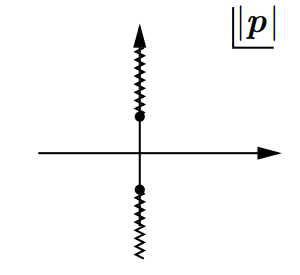
\includegraphics[scale=0.5]{Figures/branc.png}
	\caption{The branch cuts for the integral $\frac{-i}{{(2 \pi)}^{2}|x|}\int_{-\infty}^{\infty}d|p||p|e^{i|p||x|}.e^{-it\sqrt{{|p|}^{2}+{m}^{2}}}$}
\end{figure}
We term the points where the function is multivalued as branch points. Note: the starting/ending points of branch cuts needn't be branch points.

\subsection{Cauchy's Principal Value Method}
For an integral
\begin{equation}
    \int^{c}_{a} dz \ f(z)
\end{equation}
Let us suppose there exists a pole at b where $a < b < c$. How would we evaluate this? This is where we take the "principal value" $\mathcal{P}$ of the integral
\begin{equation}
    \mathcal{P} \int^{c}_{a} dz \ f(z) = \lim_{\epsilon \rightarrow 0^{+}} \left[  \int^{b- \epsilon}_{a} dz \ f(z) + \int^{c}_{b + \epsilon} dz \ f(z) \right]
\end{equation}
to obtain an unambiguous value. When we consider integrals of the form
\begin{equation}
    \int^{b}_{a} dz \ \frac{f(z)}{z + i \epsilon}
\end{equation}
where $f(z): \mathbb{C} \rightarrow \mathbb{C}$ and $a < 0 < b \in \mathbb{R}$, we use the identity
\begin{equation}
    \lim_{\epsilon \rightarrow 0^{+}} \int^{b}_{a} dz \ \frac{f(z)}{z \pm i \epsilon}  = \mathcal{P} \int^{b}_{a} dz \ \frac{f(z)}{z} \mp f(0)
\end{equation}
We then take $f(z - z_{0}) = \delta (z - z_{0})$ to obtain
\begin{equation}
    \frac{1}{z_{0} \pm i \epsilon} = \frac{\mathcal{P}}{z_{0}} \mp i \pi \delta(z_{0})
\end{equation}
\section{Group Theory}
\label{appendix_d}
\subsection{Preliminaries}
\subsubsection{Definition of a Group}
A Group is an algebraic structure i.e. a set with an operation $(G, \circ)$ which follows the axioms:
\begin{itemize}
    \item The operation is well-defined: $\forall \ a,b,c,d \in G \text{ if } a = d: a \circ b = c \implies d \circ b = c$
    \item Closure: $\forall \ a,b \in G: a \circ b \in G$
    \item Associativity: $\forall \ a,b,c \in G: a \circ (b \circ c) = (a \circ b) \circ c$	
    \item Existence of a unique Identity: $\exists \ e \in G : \forall \ a \in G: a \circ e = e \circ a =
    a$	
    \item Existence of an unique Inverse for each element: $\forall \ a \in G: \exists \  a^{-1} \in G: a \circ a^{-1} = a^{-1} \circ a = e$	
\end{itemize}
A group which displays commutativity is termed abelian and it's oppsite is called non-abelian.
\begin{figure}
	\centering
	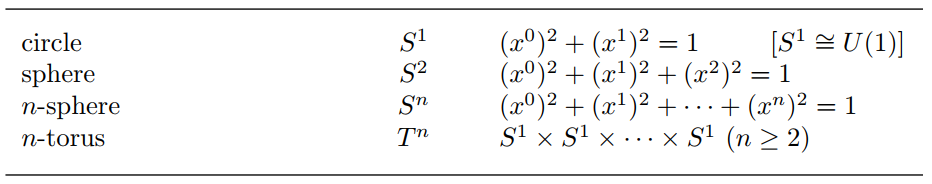
\includegraphics[scale=0.5]{Figures/Groups.png}
	\caption{Some examples of groups}
\end{figure}

\subsubsection{Subgroup}
For a group $(G, *)$, a subgroup $H \subseteq G$ is defined as a group with the same composition binary operator. The notation $H \leq G$ is often used to indicate that $H$ is a subgroup of $G$

\subsubsection{Cosets}
If $G$ is a group and $H \leq G$, then $\forall g \in G, h \in H$:
\begin{itemize}
    \item The set $g*H = {g*h}$ is termed the left coset of $H$ in $G$
    \item The set $H*g = {h*g}$ is termed the left coset of $H$ in $G$
\end{itemize}
\subsubsection{Normal Subgroup}
A subgroup $N \leq G$ whose left and right cosets are equal is termed a \textbf{normal subgroup}, denoted by $N \trianglelefteq G $
\subsubsection{Quotient Group}
For a group $G$ and a normal subgroup $N$ of $G$, the \textbf{quotient group} of $N$ in $G$, written $G/N$ and read "$G$ modulo $N$", is the set of cosets of $N$ in $G$.

\subsubsection{Morphisms}
A \textbf{group homomorphism} $\phi : G \rightarrow H$ is a map between two groups $G(G, *)$ and $H(H, +)$ that preserves the group structure i.e.
\begin{equation}
    \phi(a * b) = \phi(a) + \phi(b) \ \forall \  a,b \in G
\end{equation}
This preserves the group structure because:
\begin{itemize}
    \item This maps identity elements to identity elements i.e. $\phi(e_G) = e_{H}$
    \item $\phi(g^{-1}) = {\phi(g)}^{-1}$
\end{itemize}
The \textbf{Kernel} of a group homorphism $\phi : G \rightarrow H$ is the set of all elements of $G$ that are sent to the identity of $H$ i.e. $ker\phi = \{ g \in G | \phi(g) = e_{G}\}$
\begin{tcolorbox}
\textbf{Proposition:} A group homomorphism $\phi: G \rightarrow H$ is injective if and only if it's Kernel is trivial i.e. $ker\phi = \{ e_{G} \}$
\end{tcolorbox}
Two groups $G$ and $H$ are said to be \textbf{isomorphic} i.e. $G \cong H$ if there exists an invertible group homomorphism $\phi : G \rightarrow H$ i.e. an \textbf{isomorphism}
\begin{tcolorbox}
    \textbf{Isomorphism Theorem}\\
    Let $\phi: G \righarrow H$ be a group homomorphism. Then:
    \begin{itemize}
        \item $Im(\phi) \leq H$
        \item $Ker(\phi) \trianglelefteq G$
        \item $Im(\phi) \cong G/Ker(\phi)$
    \end{itemize}
\end{tcolorbox}
\subsection{Lie Groups}
A matrix Lie group is essentially a closed \footnote{Closed w.r.t to a topology induced from $M_{n}(\mathbb{C})$} using the operator norm\footnote{$||A|| = sup \{ \frac{||A||}{||X||} | \ X \in \mathbb{C}^{n} \textbackslash \{0\} \}$} subgroup of the general linear group\footnote{$GL(n, \mathbb{C}) = \{ A \in M_{n}(\mathbb{C}) \ | \ det(A) \neq 0\}$ i.e. the set of all linear transformations on a vector space over $\mathbb{C}$ } $G \leq GL(n, \mathbb{C})$ for some $n \in \mathbb{N}$ where, 
\begin{figure}
	\centering
	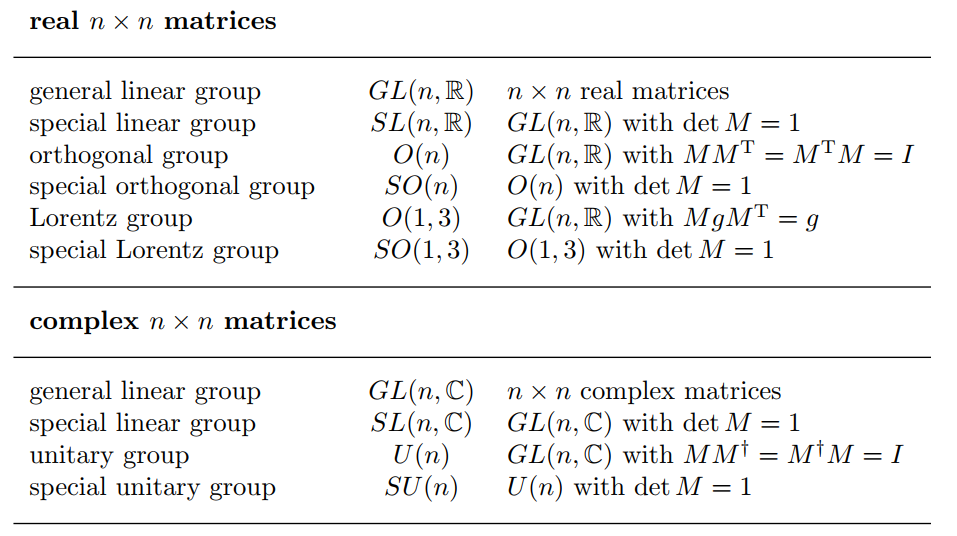
\includegraphics[scale=0.5]{Figures/Lie-Groups.png}
	\caption{Some examples of Lie groups}
\end{figure}
Some of these groups have interesting relations between them
\begin{figure}
	\centering
	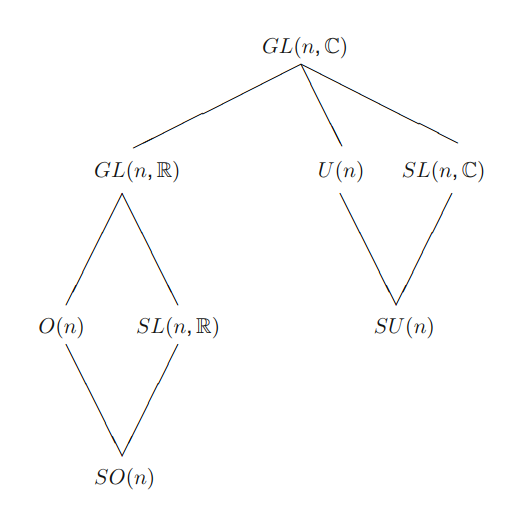
\includegraphics[scale=0.5]{Figures/cat-diag.png}
	\caption{Relationships between interesting Lie groups}
\end{figure}
\subsubsection{Generators}
We can parameterize all group elements in a form
\begin{equation}
    \left g(\alpha_{i}) \right \vert_{\alpha_{i} = 0} = e
\end{equation}
and we can consider a matrix group representation of this as
\begin{equation}
   \left  D_{n}(g(\alpha_{i})) \right \vert_{\alpha_{i} = 0} = \mathbb{I}
\end{equation}
Where we term $D_{n}$ the \textbf{representation} (we will define this clearly in the following sections) and $\mathbb{I}$ as the $n \times n$ identity matrix. Now let's take a $\delta \alpha_{i} << 1$. We can then taylor expand $D_{n}$ as,
\begin{equation}
    D_{n}(g(\delta \alpha_{i})) = \mathbb{I} + \delta \alpha_{i} \left \frac{\partial D_{n}(g(\alpha_{i}))}{\alpha_{i}} \right \vert_{\alpha_{i} = 0} + ...
\end{equation}
The leading order term is so important that we give it a label of the form
\begin{equation}
    X_{i} = -i\left \frac{\partial D_{n}(g(\alpha_{i}))}{\alpha_{i}} \right \vert_{\alpha_{i} = 0}
\end{equation}
Where $X_{i} \in M_{n}$ and the $-i \ $ has been included to ensure hermicity. Thus, we have the form \footnote{We have switched notation here, $D_{n}(g(\delta \alpha_{i})) = D_{n}(\delta \alpha_{i})$ for brevity}
\begin{equation}
    D_{n}(\delta \alpha_{i}) = \mathbb{I} + i \delta \alpha_{i} X_{i} + ...  
\end{equation}
Now if we want to consider finite transformations such as those parameterized by $alpha_{i}$, we can say that it can be constructed out of an infinite number of infinitesimal transformations
\begin{equation}
    \alpha_{i} = \lim_{N \rightarrow \infty} N \delta \alpha_{i}
\end{equation}
Thus we can rewrite in terms of our taylor expansion as\footnote{}
\begin{equation}
    \lim_{N \rightarrow \infty}{(\mathbb{I} + i \delta \alpha_{i}X_{i})}^{N} = \lim_{N \rightarrow \infty}{(\left \mathbb{I} + i \frac{\alpha_{i}}{N}X_{i} \right)}^{N}
\end{equation}
If we expand this out for several values of $N$, we will see that
\begin{equation}
    \lim_{N \rightarrow \infty}{(\left \mathbb{I} + i \frac{\alpha_{i}}{N}X_{i} \right)}^{N} = e^{i \alpha_{i}X_{i}}
\end{equation}
We call the $X_{i}$'s the \textbf{generators} of the group, which are related to the group elements through the exponential map. The number of generators of a group is termed the group's \textbf{dimension}.
\subsubsection{The Matrix exponential}
The matrix exponential is defined as,
\begin{equation}
    exp: M_{n}(\mathbb{C}) \rightarrow GL(n, \mathbb{C})
\end{equation}
for example,
\begin{equation}
    x \rightarrow \sum^{\infty}_{k=0} \frac{x^{k}}{k!}
\end{equation}
this converges for all $x$. Some interesting things about the matrix exponential:
\begin{itemize}
    \item $exp$ is surjective
    \item $e^{A. X.A^{-1}} = A e^{X}A^{-1} \ \forall \ A \in GL(n,\mathbb{C})$
    \item $det(e^{X}) = e^{tr(X)}$
    \item $e^{0} = \mathbb{I}$
    \item ${(e^{X})}^{*} = e^{X^{*}}$
    \item ${(e^{X})}^{T} = e^{X^{T}}$
    \item ${(e^{X})}^{-1} = e^{X^{-1}}$
    \item $e^{(\alpha + \beta)X} = e^{\alpha X}e^{\beta X} \ \forall \ \alpha, \beta \in \mathbb{C}$
    \item If $XY = YX$ then $e^{X + Y} = e^{X}.e^{Y} = e^{Y}.e^{X}$
    \item In general, $e^{X + Y} = \lim_{k \rightarrow \infty} (e^{X/k}.e^{Y/k})$. This is called the Lie product formula
    \item $\frac{d}{d \epsilon} e^{\epsilon X} = X e^{\epsilon X} = e^{\epsilon X} X\ \forall \epsilon \in \mathbb{R}$
    \item $\left \frac{d}{d \epsilon}  \right \vert_{\epsilon = 0 } e^{\epsilon X} = X $
    \item $e^{\epsilon X} = e^{\epsilon Y} \ \forall \ \epsilon \in \mathbb{R} \leftrightarrow X = Y$
\end{itemize}

\subsubsection{Lie Algebra}
A Lie Algebra $\mathfrak{g}$ is a vector space over some field $\mathcal{F}$ together with a binary operation $\left[,\right] := \mathfrak{g} \times \mathfrak{g} \rightarrow \mathfrak{g}$ called the Lie bracket satisfying the following axioms $\forall \ x, y,z \in \mathfrak{g} ; \forall \ a,b \in \mathcal{F}$:
\begin{itemize}
    \item \textbf{Bilinearity}
    \begin{itemize}
        \item $\left[ ax + by, z \right] = a\left[x,z\right] + b	\left[y,z\right]$
			\item $\left[ z, ax + by \right] = a\left[z,x\right] + b	\left[z,y\right]$
    \end{itemize}
    \item \textbf{Alternativity:} $\left[ x, x \right] = 0$	
    \item \textbf{Jacobi Identity:} $\left[ x, \left[ y,z \right] \right] + \left[ z, \left[ x, y \right] \right] + \left[ y, \left[ z,x \right] \right] = 0$
    \item \textbf{Anticommutativity:} $ \left[ x,y \right] = -\left[ y,x \right]$	
\end{itemize}

\subsubsection{Single-Parameter Lie groups}
A one-parameter group or one-parameter subgroup usually means a continuous group homomorphism from the real line $\mathbb{R}$ as an additive group i.e. where the group composition is addition to some other topological group G . If $\phi$ is injective then $\phi(\mathbb{R})$, the image, will be a subgroup of $G$ that is isomorphic to $\mathbb{R}$ as an additive group.
\begin{equation}
    \phi : \mathbb{R} \rightarrow G 
\end{equation}
This is how infinitesimal transformations were defined by Lie: "an infinitesimal transformation is an infinitely small transformation of the one-parameter group that it generates"

\subsubsection{Interesting things about Lie groups}
\begin{itemize}
    \item $G \leq GL(n,\mathbb{R})$ are termed compact if it is closed and bounded w.r.t. $M_{n}(\mathbb{C})$
    \item We term $G$ to be connected if for every $g \in G$ there is continuous path connecting it to the identity
    \item $G$ is termed simply connected if every loop can be shrunk to a single point i.e. no holes
    \item If $X \in \mathfrak{g}$ then $\{e^{\epsilon X} | \epsilon \in \mathbb{R}\}$ is a one parameter subgroup of $G$
    \item In fact every smooth i.e. continuous one-parameter subgroup of $G$ is of this form
    \item If $G$ is connected then every group element can be written down as an exponential map where the generators are elements of the Lie algebra
    \item All homomorphisms and isomorphisms are continuous
\end{itemize}
\subsection{Representation Theory}
A group homomorphism $\pi$ is a representation if it's domain is $GL(V)$ for some vector space $V$ 
\begin{equation}
    \pi: G \rightarrow GL(V)
\end{equation}
For all $g \in G$, two representations $\pi_{1}(g) \rightarrow V_{1}$ and $\pi_{2}(g) \rightarrow V_{2}$ are considered \textbf{equivalent} if there is a matrix $A: V \rightarrow V$ such that
\begin{equation}
    \pi_{1}(g) = A^{-1} \pi_{2}(g) A
\end{equation}
 Here, $A$ is termed a \textbf{similarity transform}. Let's say we have two representations $\pi_{1}: G \rightarrow V_{1}$ and $\pi_{2}: G \rightarrow V_{2}$, we can then define a new representation $\pi$ of the form
\begin{equation}
    (\pi_{1}\oplus\pi_{2})(g) = \pi_{1}(g)\oplus\pi_{2}(g) = \begin{pmatrix}
\pi_{1}(g) & 0 \\
0 & \pi_{2}(g)
\end{pmatrix}
\end{equation}
This matrix form is often called the block-diagonal form. In the above example and are called the sub-representations of $\pi$. An \textbf{irreducible representation} (often called an “irrep”) is a representation with no sub-representations (except for the trivial one and itself).
%\subsection{Important Theorems}
%\subsubsection{Lagrange's Theorem}
%\begin{tcolorbox}
 %   For any finite group G, the order (number of elements) of every subgroup of G is  equal to the number of of left cosets of $H$ in $G$
%\end{tcolorbox}
%\subsubsection{Cayleys's Theorem}
%\begin{tcolorbox}
 %   Every group $G$ is isomorphic to a subgroup of the symmetric group acting on $G$
%\end{tcolorbox}
%\subsubsection{Schur's Lemma}
%\begin{tcolorbox}
    
%\end{tcolorbox}
\section{Variational Calculus}
\subsection{A Lemma}
If,
\begin{equation}
    \int_{a}^{b}A(t)\eta(t)dt =0
\end{equation}
where,
\begin{itemize}
    \item $\eta(a) = \eta(b) = 0$
    \item $A(t)$ and $\eta(t)$ are both twice differentiable in the closed interval $[a,b]$ 
\end{itemize}
then,
\begin{tcolorbox}
$A(t) = 0$ throughout $[a,b]$
\end{tcolorbox}
\subsubsection{Proof by Contradiction}
Suppose that there exists $A(c) \neq 0$ for some $a < c < b$. For definiteness let's also suppose that $A(c) > 0$. Due to the continuity of $A(t)$, an interval $[t_{1},t_{2}]$ about c but within $[a,b]$ exists on which A(t) > 0. However under these conditions we can construct a $\eta(t)$ that leads to the integral being non-zero. For example,
\begin{equation} \label{deltadef}
\eta(t) =  
\begin{cases}
{(t-t_{1})}^{3}{(t_{2}-t)}^{3}, & \text{for } t_{1} < t < t_{2}\\
0, & \text{for } t < t_{1} \text{ and } t > t_{2}
\end{cases}
\end{equation}
this $\eta(t)$ has continuous second derivative throughout $[a,b]$ and meets the stated boudary conditions , however the integral does not vanish contrary to the statement. To prevent this thus, it must be $A(t)$ that must vanish throughout $[a,b]$.

\subsection{Deriving the Euler-Lagrange Equations}
The goal here is to find the extremal of the functional
\begin{equation}
			J(\alpha) = \int_{x_{2}}^{x_{1}}f\{y(\alpha , x),y^{'}(\alpha , x);x \} dx
		\end{equation}
		That is $\forall \ \eta(x)$, we want to find
		\begin{equation}
		\left. \frac{\partial J}{\partial \alpha} \right |_{\alpha = 0}  = 0
		\end{equation}
		Where $\alpha$ is a parameter.We thus start by, parameterizing $y$ as,
		\begin{equation} \label{increment}
		    y(x) = y(0) + \alpha \eta(x)
		\end{equation}
\begin{figure}
	\centering
	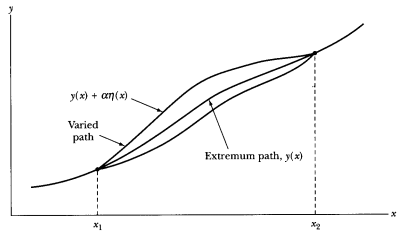
\includegraphics[scale=0.8]{Figures/var.png}
	\caption{We can think of this as trying to find the extremized path from a perturbed one}
\end{figure}
	We can now take the derivative
\begin{equation}
\frac{\partial J}{\partial \alpha} = \frac{\partial}{\partial \alpha}\int_{x_{2}}^{x_{1}}f\{y(\alpha , x),y^{'}(\alpha , x);x \} dx
\end{equation}
\begin{equation} \label{eq-varpar}
    \frac{\partial J}{\partial \alpha} = \int_{x_{2}}^{x_{1}} \left(\frac{\partial f}{\partial y}\frac{\partial y}{\partial \alpha} + \frac{\partial f}{\partial y^{'}}\frac{\partial y^{'}}{\partial \alpha} \right) dx
\end{equation}
From Equation (\ref{increment}) we have
\begin{align}
\frac{\partial y}{\partial \alpha} = \eta(x) \ ; \  & \frac{\partial y^{'}}{\partial \alpha} = \frac{d \eta}{d x}
\end{align}
Plugging this back in to equation (\ref{eq-varpar})
	$$\frac{\partial J}{\partial \alpha} = \int_{x_{2}}^{x_{1}} \left(\frac{\partial f}{\partial y}\eta(x) + \frac{\partial f}{\partial y^{'}}\frac{\partial \eta}{\partial x} \right) dx$$	
	The second term in the integrand can be integrated by parts:
	$$\int_{x_{1}}^{x_{2}} \frac{\partial f}{\partial y^{'}}\frac{d \eta}{dx} dx = \left \frac{\partial f}{\partial y^{'}} \eta(x) \right |^{x_{2}}_{x_{1}} -\int_{x_{1}}^{x_{2}} \frac{d}{dx} \left(\frac{\partial f}{\partial y^{'}}\right)\eta(x) dx $$
	$$\frac{\partial J}{\partial \alpha} = \int_{x_{1}}^{x_{2}} \left(\frac{\partial f}{\partial y} - \frac{d}{dx}\frac{\partial f}{\partial y^{'}} \right) \eta(x) dx$$
	\begin{tcolorbox}
		\begin{equation}
		\frac{\partial f}{\partial y} - \frac{d}{dx}\frac{\partial f}{\partial y^{'}} = 0
		\end{equation}
	\end{tcolorbox}
\subsection{Special Notation}
	We have the equation
\begin{equation}
\frac{\partial J}{\partial \alpha} d\alpha = \int_{x_{1}}^{x_{2}} \left(\frac{\partial f}{\partial y} - \frac{d}{dx}\frac{\partial f}{\partial y^{'}} \right) \frac{\partial y}{\partial \alpha} d \alpha dx = 0
\end{equation}
It can be written as 
\begin{equation}
\delta J = \int_{x_{1}}^{x_{2}} \left(\frac{\partial f}{\partial y} - \frac{d}{dx}\frac{\partial f}{\partial y^{'}} \right) \delta y \ dx = 0
    \end{equation}
where
\begin{equation}
\begin{cases}
\frac{\partial J}{\partial \alpha} d\alpha = \delta J\\
\frac{\partial y}{\partial \alpha} d\alpha = \delta y
\end{cases}
\end{equation}
The condition of extremum then becomes,
\begin{equation}
\delta J = \delta \int_{x_{1}}^{x_{2}} f\{y, y^{'}; x\} dx = 0
\end{equation}
Sometimes we term this the functional derivative i.e. the Frechet derivative
\begin{equation}
    \frac{\delta J}{\delta y} = \frac{\partial f}{\partial y} - \frac{d}{dx}\frac{\partial f}{\partial y^{'}}
\end{equation}

\subsection{The Legendre Transform}
The Legendre transform is way of renaming the dependent variables of a functional. For example, consider the following function $f(x,y)$ whose total derivative is
\begin{equation}
    df = \frac{\partial f}{\partial x}dx + \frac{\partial f}{\partial y}dy 
\end{equation}
Now let's define a new function $g(x,y,u)$, whose total derivative looks like
\begin{equation}
    dg = d(ux) - df = udx + xdu - \frac{\partial f}{\partial x}dx - \frac{\partial f}{\partial y}dy
\end{equation}
However if we define,
\begin{equation}
    u(x,y) = \frac{\partial f}{\partial x}
\end{equation}
Then the term proportional to $dx$ vanishes i.e. we get
\begin{equation}
    dg = xdu - \frac{\partial f}{\partial y}dy
\end{equation}
We can thus consider $g$ as simply a function of  $u$ and $y$ by defining $x := x (u,y)$ that is
\begin{equation}
    g(u,y) = ux(u,y) - f(x(u,y),y)
\end{equation}
This is called the Legendre transform. It takes one function to another by renaming one of it's dependent variable's derivatives. However we haven't lost any information about the original function, as from the identities
\begin{equation}
    \begin{align}
        \left \frac{\partial g}{\partial u} \right |_{y} = x(u,y) \ \ \text{and} \ \ \left \frac{\partial g}{\partial y} \right |_{u} =  -\frac{\partial f}{\partial y}
    \end{align}
\end{equation}
we can get back the original function through the inverse Legendre transform $f = (\partial g/ \partial u)u - g$
\section{Probability Distributions}
\subsection{Discrete Distributions}
Suppose we have a frequency distribution 
\begin{equation}
N = \sum_{j=0}^{\infty} N(j)
\end{equation}
The probability of an event $N_{j}$ is defined as,
\begin{equation}
P(j) = \frac{N(j)}{N}
\end{equation}
In probability theory, the sum of all probabilities is 1,
\begin{equation}
\sum_{j = 0}^{\infty}P(j) = \sum_{j = 0}^{\infty}\frac{N(j)}{N} = 1
\end{equation}
The average/mean/expectation value of a value $j$ is given by the formula:
\begin{equation}
	\expval{j} = \frac{\sum j N(j)}{N} = \sum_{j =0 }^{\infty} j P(j)
\end{equation}
and in general, the average of some function of $j$, is given by,
\begin{equation}
\expval{f(j)} = \sum_{j =0 }^{\infty} f(j) P(j)
\end{equation}
The spread of a variable's value from it's mean is called it's variance, written as
\begin{equation}
\sigma^{2} = \expval{{(\Delta j)}^{2}}
\end{equation}
where,
$$\Delta j = j - \expval{j}$$
It's square root is called the standard deviation,
\begin{equation}
\sigma = \sqrt{\expval{{(\Delta j)}^{2}}} =  \sqrt{\expval{j^{2}} - \expval{j}^{2}}
\end{equation}
Which comes from a theorem on variances that we'll find useful later on:
$$\sigma^{2} = \expval{{(\Delta j)}^{2}} = \sum {(\Delta j)}^{2} P(j) = \sum {(j- \expval{j})}^{2} P(j)$$
$$ = \sum (j^{2} - 2j \expval{j} + \expval{j}^{2}) P(j)$$
$$ = \sum j^{2}P(j) - 2 \expval{j} \sum jP(j) + \expval{j}^{2}\sum P(j)$$
$$ = \expval{j^{2}} - 2 \expval{j}\expval{j} + \expval{j}^{2} = \expval{j^{2}} - \expval{j}^{2}$$
\subsection{Continuous Distributions}
We now move to a continuous probability distribution, we'll create continuous analogs of all the quantities we just introduced. Let's start with probability, the probability of that $x$ lies between $a$ and $b$
\begin{equation}
	P_{ab} = \int_{a}^{b} \rho(x) dx
\end{equation}
where $\rho(x)$ is the called the probability density i.e. the probability of getting $x$, or more concretely,
$$\rho(x)dx = \text{Probability that an individual is chosend at random lies between } x \text{ and } x + dx$$
Now supposing the rules we held for discrete variables hold, the continuous analogs look like this:
\begin{equation}
	1 = \int_{- \infty}^{\infty} \rho(x) dx
\end{equation}
\begin{equation}
	\expval{x} = \int_{- \infty}^{\infty} x \rho(x) dx
\end{equation}
\begin{equation}
	\expval{f(x)} = \int_{- \infty}^{\infty} f(x) \rho(x) dx
\end{equation}
\begin{equation}
	\sigma^{2} := \expval{(\Delta x)^{2}} = \expval{x^{2}} - {\expval{x}}^{2}
\end{equation}
%\section{Expectation Values}
%In this section we'll explore how we express the expectation values of a few opeartors. Let's start with the position opeartor in the position representation (i.e. position basis):
%\begin{equation} \label{posex}
	%\expval{x} = \int_{- \infty}^{\infty} x \abs{\psi(\vec{x}, t)}^{2} dx
%\end{equation}
%We can differentiate \ref{posex} with respect to time to find the expectation value for "velocity":
%$$\frac{d \expval{x}}{dt} = $$
%Throwing away 
%\begin{equation}
%	\expval{v} = \frac{d \expval{x}}{dt} = -\frac{i \hbar}{m} \int \psi^{*} \frac{\partial \psi}{\partial x} dx
%\end{equation}
%Therefore we can write the expectation value of momentum as,
%\begin{equation}
%	\expval{p} = m \frac{d \expval{x}}{dt} =  -i \hbar \int \left(\psi^{*} \frac{\partial \psi}{\partial x} \right) dx
%\end{equation}
%In general, every observable is a function of position and momentum, thus for an observable %$\hat{O}(x,p)$, the expectation value is given by,
%\begin{equation}
%	\expval{\hat{O}(x,p)} = \int \psi^{*} \hat{O}(x,-i \hbar \nabla) \psi dx
%\end{equation}
%For example, the expectation value of kinetic energy is,
%\begin{equation}
%\expval{T} = -\frac{\hbar^{2}}{2m} \int \psi^{*} \frac{\partial^{2} \psi}{\partial x^{2}} dx
%\end{equation}
%Or to sum it up in Dirac notation,
%\begin{equation}
%	\expval{\hat{O}} = \expval{\hat{O}}{\psi}
%\end{equation}

\section{Covariant Derivative}
A connection is a tool that allows us to compare prices or phases at different locations since
it keeps track of how the local coordinate systems are defined and encodes information about
the structure of the space we are moving in.
As already mentioned above, there are two situations where it’s necessary to introduce
connections. One the one hand, we need connections to allow arbitrary local coordinate
systems. Here the connection keeps track of these local coordinate systems and lets us
compare prices or phases defined according to different local conventions. On the other
hand, connections are essential whenever the space we are interested in is curved.
The prototypical example of a curved space is a sphere. To compare vectors at two different
points on a sphere (e.g. to calculate a derivative), we need a procedure to move one vector
to the location of the second one consistently.
The needed procedure is known as parallel transport. To understand it imagine we can
imagine that we are walking on the sphere while holding a stick in your hand. While we are
walking we our best to keep the stick straight. If we do this, we are parallel transporting
the stick.
Mathematically, the infinitesimal parallel transport of a vector Vα(x) is defined as
\begin{equation}
V_{\alpha}(x + dx) = V_{\alpha}(x) - \Gamma^{\alpha}_{\beta \gamma}(x)V^{\beta}(x)dx^{\gamma}
\end{equation}
    where $\Gamma^{i}_{jk}$ denotes the corresponding connection.
An important observation is that if the space we are moving in is curved, it’s possible
the stick does not end up in its starting position if we move along a closed curve.
\begin{figure}[!ht]
	\centering
	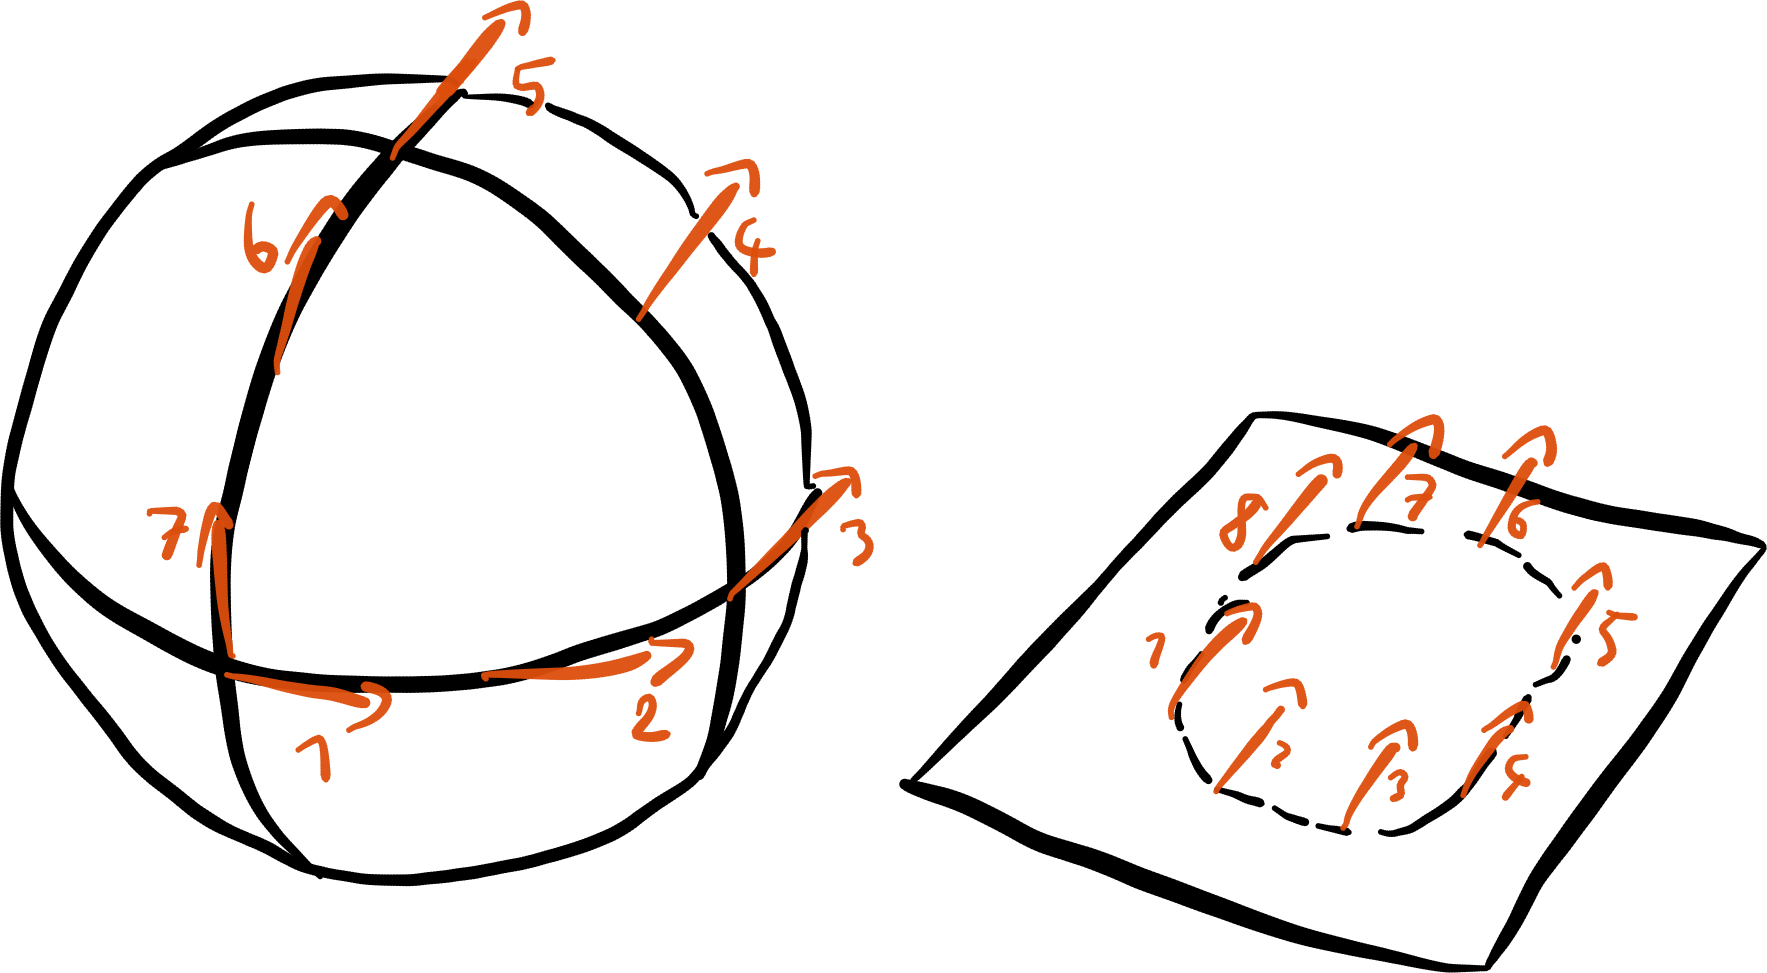
\includegraphics[scale=0.2]{Figures/23-2.png}
	\caption{A pictorial representation of Parallel Transport}
\end{figure}
Hence, the difference between the original vector and the vector which was parallel transported along an infinitesimal closed curve encodes information about the local curvature.
Therefore, to define curvature we imagine that our vector moves from A to B via two different paths.
\begin{figure}[!ht]
	\centering
	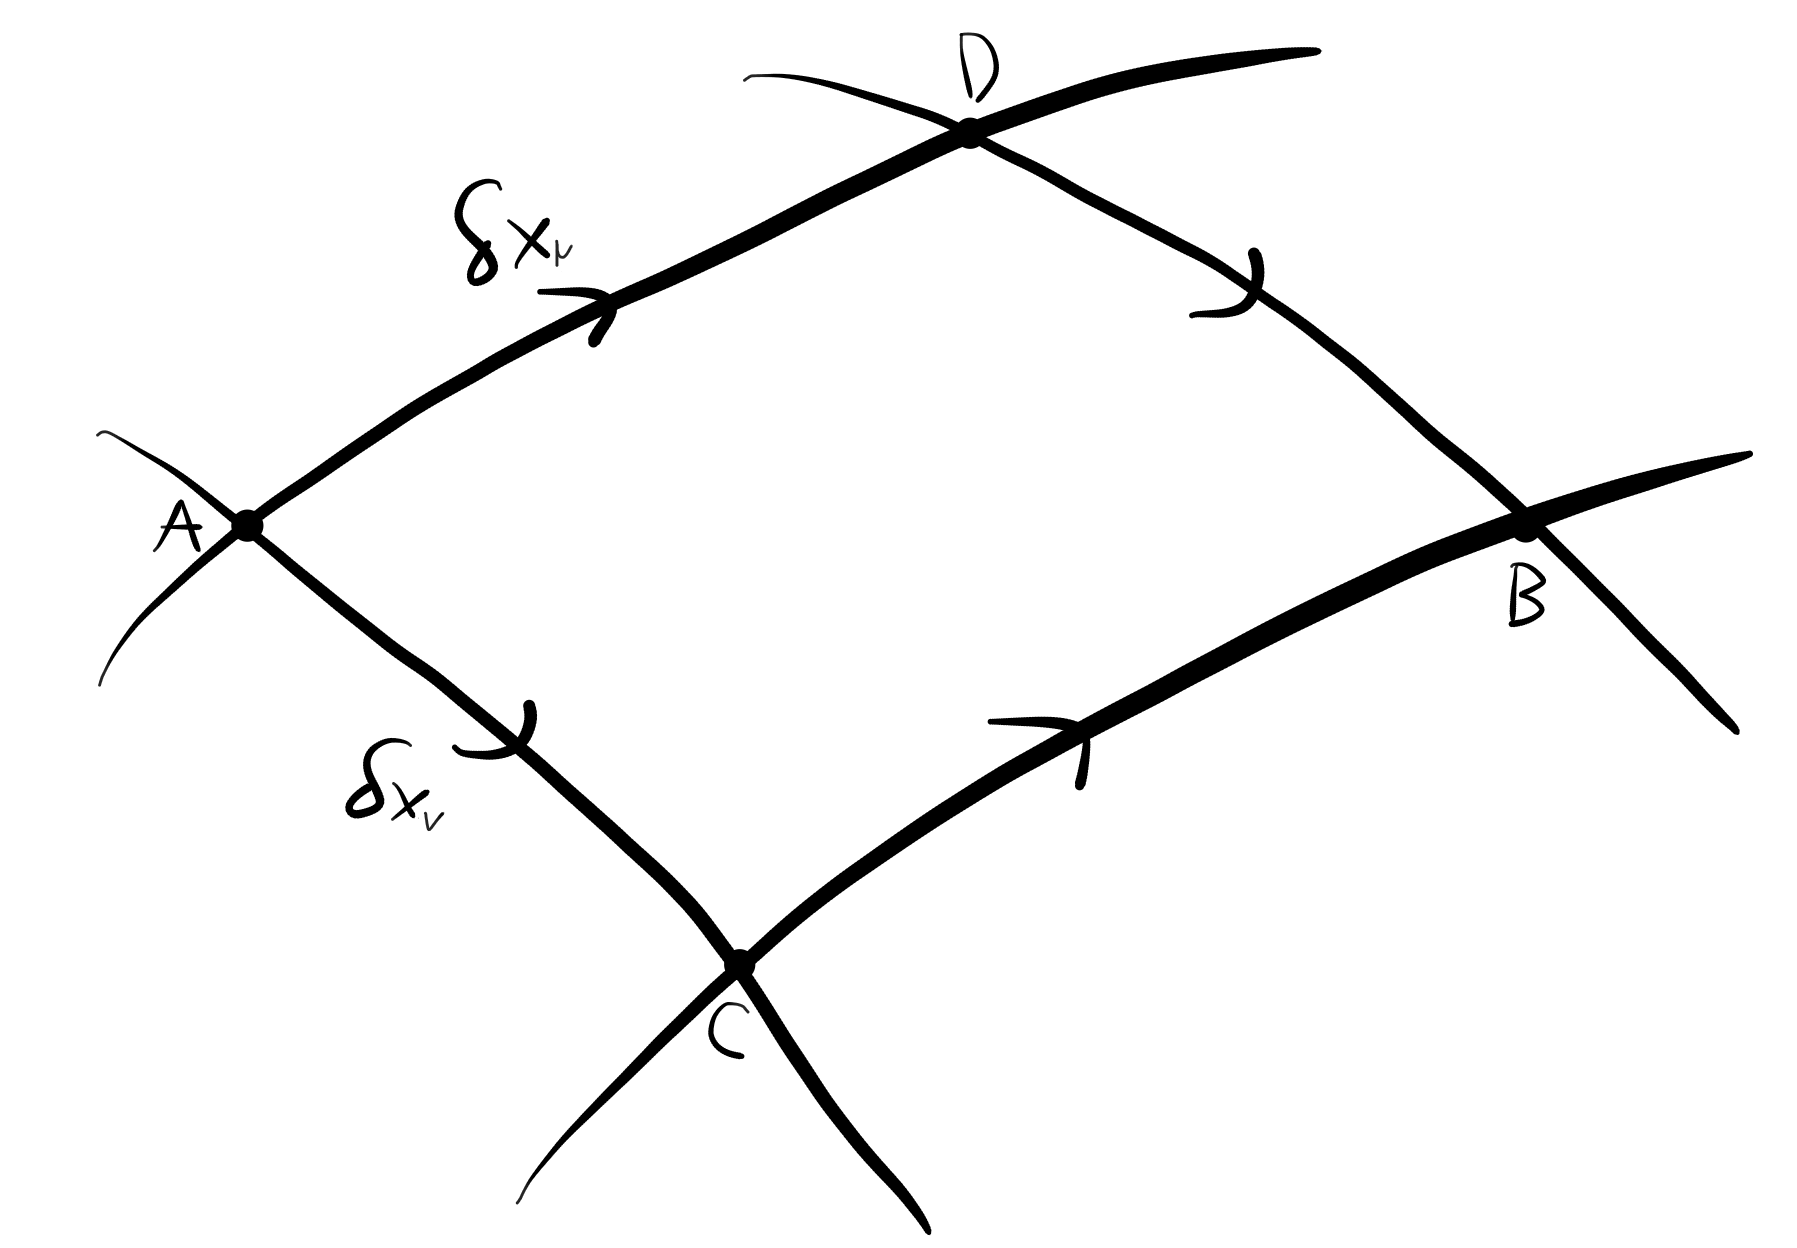
\includegraphics[scale=0.5]{Figures/curvatureloop.png}
	\caption{A pictorial representation of taking two different paths}
\end{figure}
Taken together these two paths yield a closed curve and we can calculate
\begin{equation}
    V_{\alpha}(A \rightarrow C \rightarrow B)  - V_{\alpha}(A \rightarrow D \rightarrow B) = R^{\gamma}_{\alpha \beta \mu}V^{\beta}dx^{\mu}dx^{\nu}
\end{equation}
where $R^{\nu}_{\alpha \beta \mu}$
denotes the corresponding (Riemann) curvature tensor
\begin{equation}
    R^{\nu}_{\alpha \beta \mu} =  \partial_{\alpha}\Gamma^{\mu}_{\beta \nu} - \partial_{\beta}\Gamma^{\mu}_{\alpha \nu} + \Gamma^{\mu}_{\alpha \kappa}\Gamma^{\kapa}_{\beta \nu} - \Gamma^{\mu}_{\beta \kappa}\Gamma^{\kappa}_{\alpha \nu}
\end{equation}
\subsection{The Formalism}
The covariant derivative of a vector field $v^{\mu}$ is defined as,
\begin{equation}
\nabla_{\mu} v^{\alpha} = v^{\alpha}_{ \  ; \mu} = \partial_{\mu} v^{\alpha} + \Gamma^{\alpha}_{\mu \nu} v^{\nu}
\end{equation}
 It is worth noting that the connection i.e. theChristoffel symbol is not a tensor because it contains all the information about the curvature of the coordinate system and can therefore be transformed entirely to zero if the coordinates are straightened. Nevertheless we treat it as any ordinary tensor in terms of the index notation. It can be defined in terms for derivatives as:
\begin{equation}
\Gamma^{k}_{ij}\vec{e}_{k} = \frac{\partial \vec{e}_{i}}{\partial x^{j}}
\end{equation}
Where, the index $i$ specifies the basis vector for which the derivative is being
taken, the index $j$ denotes the coordinate being varied to induce this change
in the $i$th basis vector, and the index $k$ identifies the direction in which this
component of the derivative points. We define the Christoffel symbol in terms of the metric $g_{\mu \nu}$ and it's inverse $g^{\alpha \beta}$ as\footnote{The connection coefficients defined here are of the Levi-Civita Connection. It a unique connection (covariant derivative) that is Torsion-Free and has Metric Compatibility},
\begin{equation}
\Gamma^{\alpha}_{\ \mu \nu} = \frac{1}{2} g^{\alpha \beta} \left(\frac{\partial g_{\beta \nu}}{\partial x^{\mu}} + \frac{\partial g_{\beta \mu}}{\partial x^{\nu}} - \frac{\partial g_{\mu \nu}}{\partial x^{\beta}}\right) = \frac{1}{2}g^{\alpha \beta} \left(g_{\beta \nu, \mu} + g_{\beta \mu, \nu} - g_{\mu \nu, \beta}\right)
\end{equation}
We can then define the covariant derivative of a covector as,
\begin{equation}
\nabla_{\mu} w_{\alpha} = w^{\alpha}_{ \  ; \mu} = \partial_{\mu} w_{\alpha} + \Gamma^{\alpha}_{\mu \nu} w_{\nu}
\end{equation}
The covariant derivative of a tensor $t^{\alpha\beta}$ is then,
\begin{equation}
\nabla_{\mu}t^{\alpha \beta} = \partial_{\mu} t^{\alpha \beta} + \Gamma^{\alpha}_{\mu \sigma}t^{\sigma \beta} + \Gamma^{\beta}_{\mu \sigma}t^{\alpha \sigma }
\end{equation}
and of a tensor $t^{\alpha}_{\beta}$,
\begin{equation}
\nabla_{\mu}t^{\alpha}_{\beta} = \partial_{\mu} t^{\alpha}_{\beta} + \Gamma^{\alpha}_{\mu \sigma}t^{\sigma}_{\beta} + \Gamma^{\beta}_{\mu \sigma}t^{\alpha}_{\sigma}
\end{equation}